%!TEX program = xelatex
% 完整编译: xelatex -> bibtex -> xelatex -> xelatex

\documentclass[lang=cn,11pt,a4paper,cite=authoryear]{elegantpaper}
\usepackage{indentfirst}
\setlength{\parindent}{2em}

\title{编译原理实验二:语义分析}
\author{林搏海 1190202128}
\institute{{哈尔滨工业大学} {物联网工程}}
\date{\zhtoday}


% 本文档命令
\usepackage{array}
\newcommand{\ccr}[1]{\makecell{{\color{#1}\rule{1cm}{1cm}}}}

\begin{document}

\maketitle

\begin{abstract}
\hspace*{0.7cm}我们在Lad1实现的基于Flex的词法分析和基于Bison的语法分析的基础上,实现了语法制导的语义翻译过程,对于c--代码的常见语义错误进行了检测和错误提示输出,除了对于实验指导书上基本语法错误的检测之外,我们还实现了选做二的错误检测,即对于变量作用域的限制,并且输出相应的错误信息。为了实现这些新增功能,我们建立了基于十字链表的哈希表结构用于存储和查询符号,使其能够在对于符号进行高效插入删除和检索的基础之上,还能够支持对于符号作用域的标注和限制。
\keywords{语法分析树, Flex, Bison, 十字链表, 哈希表}
\end{abstract}



\section{语义分析}
\subsection{语义分析过程概述}
我们通过遍历实验一中的语法分析树来进行语义分析,语义分析主要是对于出现的符号进行一系列的类型检测工作,因此,当我们遇到一个需要处理的符号的时候,此时遍历语法分析树的过程一定是进入了ExtDef之后,因此我们每一次遇到ExtDefen就会进行对应的语法分析,然后对其递归地展开,就可以对于所有的非终结符进行处理,并且对于符号表进行操作和相应的语义错误检测。

\subsection{符号表原理及其实现}
在遍历语法分析树进行语义分析的时候,我们需要通过符号表来记录所有的符号出现过的位置,类型等信息,并且符号表还需要支持高效的查找和插入删除,同时,我们还希望符号表可以区分不同作用域的符号,以此来完成实验选做二。因此,我们选用了哈希表加上十字链表的机制来实现符号表,其中,通过哈希表来实现符号的快速增删查,通过把同一作用域的符号串联起来的形式来实现对于符号作用域的识别。
对于符号表的哈希结构和十字链表,我们进行了如下的定义如图\ref{pic1}
\begin{figure}[h]
	\centering
	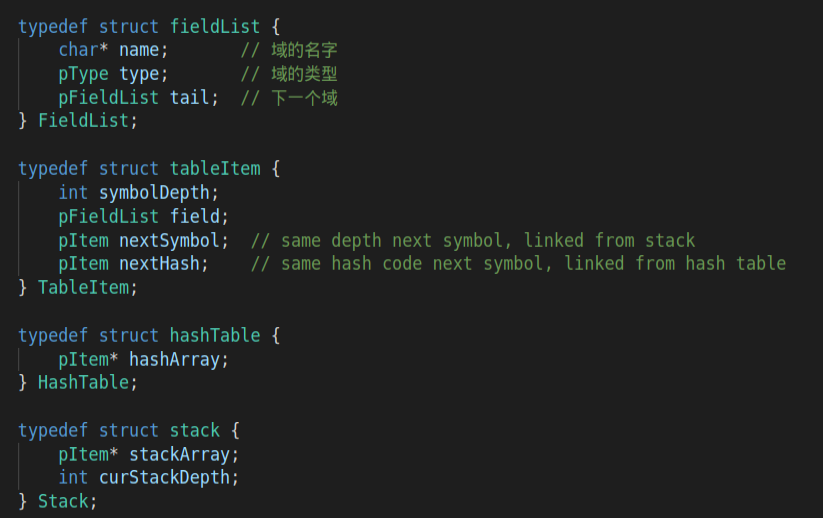
\includegraphics[width=\textwidth]{pics//11.png}
	\caption{符号表定义}
	\label{pic1}
\end{figure}

此外,为了方便区分函数符号以及结构体,我们对于结构体和函数信息进行了存储,对于匿名结构体,因
为词法分析中规定了 id 不能为纯数字,所以此处我们用数字编号作为匿名结构体的名字,可以避免与其他符号的命名冲突,数字编号通过在table结构体中记录匿名结构体的个数来获得编号。

我们对于LR(1)文法中的产生式编写了过程,在检测到对应的错误的时候会输出错误信息。如图\ref{pic2}
\begin{figure}[h]
	\centering
	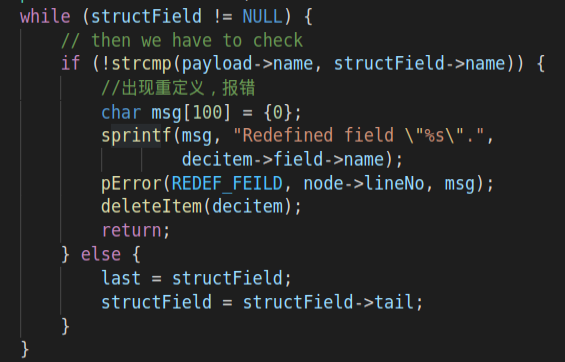
\includegraphics[height=6.5cm,width=10cm]{pics//22.png}
	\caption{错误输出}
	\label{pic2}
\end{figure}

此外,为了进行空间管理,防止出现内存泄漏的情况,我们对于哈希表空间进行了严格的释放流程,当一个域结束之后,我们释放当前域中声明的符号,当程序运行结束的时候,我们释放所有的空间。图\ref{pic3}
\begin{figure}[h]
	\centering
	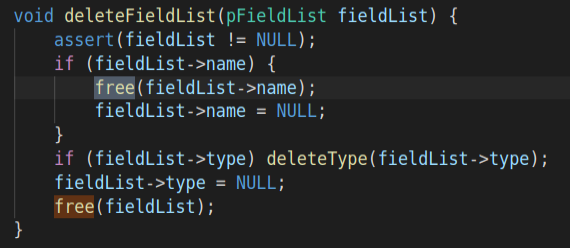
\includegraphics[width=\textwidth]{pics//33.png}
	\caption{空间释放}
	\label{pic3}
\end{figure}



\section{主程序模块}
为了方便编译和调试,我们将main函数放在了main.c文件中,其具体逻辑入下:首先,读入我们的cmm文件,调用yyparse()函数对其进行词法分析和语法分析,并且建立相应的语法分析树。如果词法分析阶段或者是语法分析阶段检测到错误,那么我们就调用我们自己重写的error函数进行报错;如果此过程没有错误,那么我们就初始化符号表,并且从根节点开始遍历整个语法分析树,并且执行对应的分析语句,如果出现语义错误,则输出相应的错误类型,如果整个程序没有任何的词法语法或者是语义错误,那么就不输出任何信息,并且在退出程序时释放语法分析树和符号表的空间。
\section{编译执行方式}
程序的正确编译执行需要以下八个文件:enum.h, node.h, lexical.l, main.c, syntax.y, makefile, semantic.h, semantic.c, 只需要确保他们处在同一个目录下,然后执行make命令调用makefile文件执行自动编译即可。

\end{document}
